\noindent Myonen, Elektronen und Tauonen bilden zusammen mit ihren jeweiligen
Neutrinos im Standardmodell der Elementarteilchen die Familie der Leptonen. Alle
genannten Teilchen besitzen einen halbzahligen Spin. Das Myon, das Elektron
sowie das Tauon tragen zusätzlich die Elementarladung, während ihre Neutrinos
ungeladen sind. \\
\FloatBarrier
\begin{figure}
  \centering
  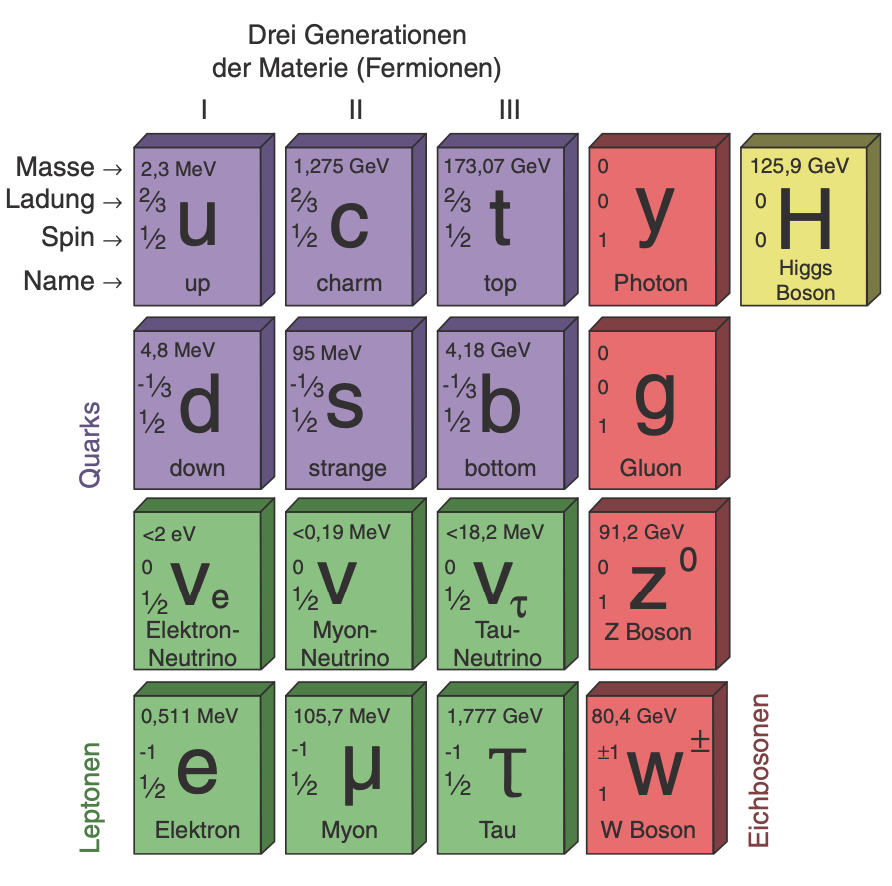
\includegraphics[scale=0.5]{resources/standardmodell.png}
  \caption{Fermionische Elementarteilchenfamilien mit ihren zugehörigen
  Wechselwirkungsbosonen und dem Higgs-Boson \cite{großforschung}.}
  \label{fig:01}
\end{figure}
\FloatBarrier
\subsubsection{Entstehung und Zerfall von Myonen}
\noindent Beim Zerfall geladener Pionen $\pi^{\pm}$ in den oberen Schichten
der Erdatmosphäre in einer Höhe von etwa $\SI{15}{\kilo\meter}$ entstehen
geladene Myonen gemäß den Zerfallsgleichungen \ref{eqn:01} \cite{grupen}.
\begin{align}
  \ce{\symup{\pi}+ -> \symup{\mu}+ + \symup{\nu}}, \qquad
  \ce{\symup{\pi}- -> \symup{\mu}- + \bar{\symup{\nu}}}.
  \label{eqn:01}
\end{align}
\noindent Die entstehenden Myonen sind allerdings nicht stabil und zerfallen
unter der schwachen Wechselwirkung
mit einer mittleren Lebensdauer von etwa $\tau = \SI{2.2}{\micro\second}$ in
ein Elektron und ein Elektron-Antineutrino (für $\ce{\symup{\mu}- }$) bzw.
ein Positron und ein Elektron-Neutrino (für $\ce{\symup{\mu}+ }$) mitsamt ihrer
jeweiligen Myon-Antineutrinos bzw. Myon-Neutrinos, ohne dabei die
Leptonenzahlerhaltung zu verletzen \cite{grupen}. \\
\newline
\noindent Eine klassische Betrachtung der möglichen freien Weglänge der Myonen
bis zu ihrem Zerfall zeigt schnell, dass diese selbst unter der Annahme, dass
sie sich mit Lichtgeschwindigkeit fortbewegen, maximal eine Strecke von zirka
$s_0 = \SI{660}{\meter}$ zurücklegen können. Der scheinbare Widerspruch, dass Myonen
auf der Erdoberfläche detektiert werden können löst sich erst unter
Berücksichtigung relativistischer Effekte. So beträgt die zurückgelegte Strecke
im Ruhesystem der Myonen aufgrund der Längenkontraktion unter der Annahme einer
mittleren Geschwindigkeit der Myonen von $\bar{v}_\text{Myon} = 0.9999 \cdot c$
etwa
\begin{align}
s =\frac{1}{\sqrt{\left(1 - \frac{{v_\text{Myon}}^2}{c^2} \right)}} \cdot s_0 \approx \SI{46.7}{\kilo\meter}.
\label{eqn:02}
\end{align}
\noindent Um die Lebensdauer kosmischer Myonen zu ermitteln, ist es erforderlich,
sowohl die Myonen, als auch ihren Zerfall eindeutig zu detektieren. Myonen
zerfallen schwach wechselwirkend über ein W-Boson in ein Positron bzw. Elektron
(je nach Ladung des zerfallenden Myons) und die zugehörigen Neutrinos der
jeweiligen Leptonenfamilien \cite{grupen}. Für den Versuch ist es daher
erforderlich, sowohl Myonen zu erkennen, als auch diese eindeutig von
zerfallenden Myonen unterscheiden zu können. Registriert werden die Myonen in
einem Szintillatortank mit angeflanschten Photomultipliern (PMT),
Zerfallscharakteristika werden durch eine elektrische Schaltung wie in Abbildung
\ref{fig:02} untersucht. \\
\FloatBarrier
  \begin{figure}
    \centering
    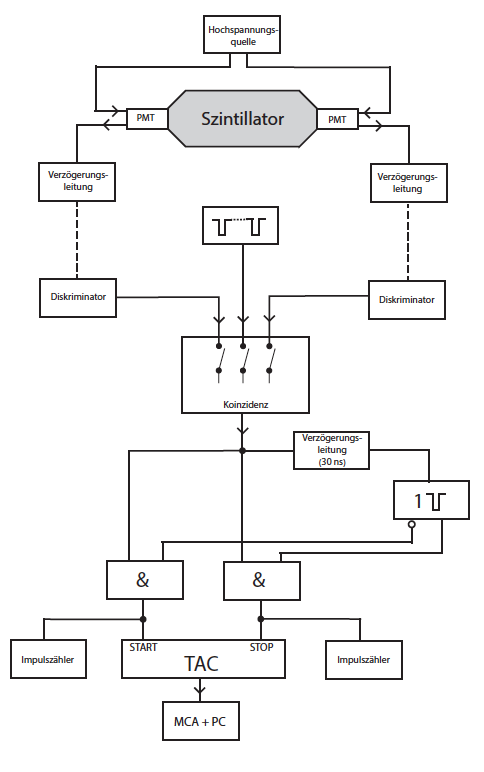
\includegraphics[scale=0.7]{resources/schaltplan.png}
    \caption{Schaltplan des Versuchsaufbaus}
    \label{fig:02}
  \end{figure}
  \FloatBarrier
\subsubsection{Szintillationsdetektoren}
\noindent Die Detektion von Myonen erfolgt unter Ausnutzung einer besonderen
Form der Lumineszenz, der Szintillation. Bei der Szintillation wird je nach
Detektormaterial innerhalb einer organischen oder anorganischen Substanz ein
Teil der beim Durchgang geladener Teilchen absorbierten Energie in Form von
Photonen wieder freigesetzt. Diese Photonen selbst sind zu niederenergetisch, um
Folgereaktionen im Szintillator auszulösen. Die Lichtsignale gelangen dann durch
das für die emittierten Photonen transparente Material zu Photodetektoren (PMTs) und
werden dort weiterverarbeitet. Der Unterschied zwischen organischen und
anorganischen Szintillatoren liegt darin, dass organische Szintillatoren
Lichtsignale sehr schnell weiterleiten, während anorganische Szintillatoren
eine verbesserte Energieauflösung zeigen \cite{szintillatoren}.
\subsubsection{Photomultiplier}
\noindent Abbildung \ref{fig:03} zeigt den schematischen Aufbau eines PMTs.
Angeflanscht an den Szintillatortortank lösen die ankommenden Photonen
Elektronen aus einem Photokathodenmaterial, welche durch eine angelegte
Hochspannung zu Dynoden beschleunigt werden. Dort lösen die Elektronen weitere
Sekundärelektronen aus und werden gemeinsam mit diesen zur nächsten Dynode
beschleunigt. Treffen die Elektronen, deren Anzahl auf ein Vielfaches der
ursprünglich anregenden Elektronen angestiegen ist anschließend auf eine Anode,
kann dieser Strom als Signal gemessen werden und als im Szintillatortank
registriertes Myon interpretiert werden \cite{pmt}. \\
\FloatBarrier
\begin{figure}
  \centering
  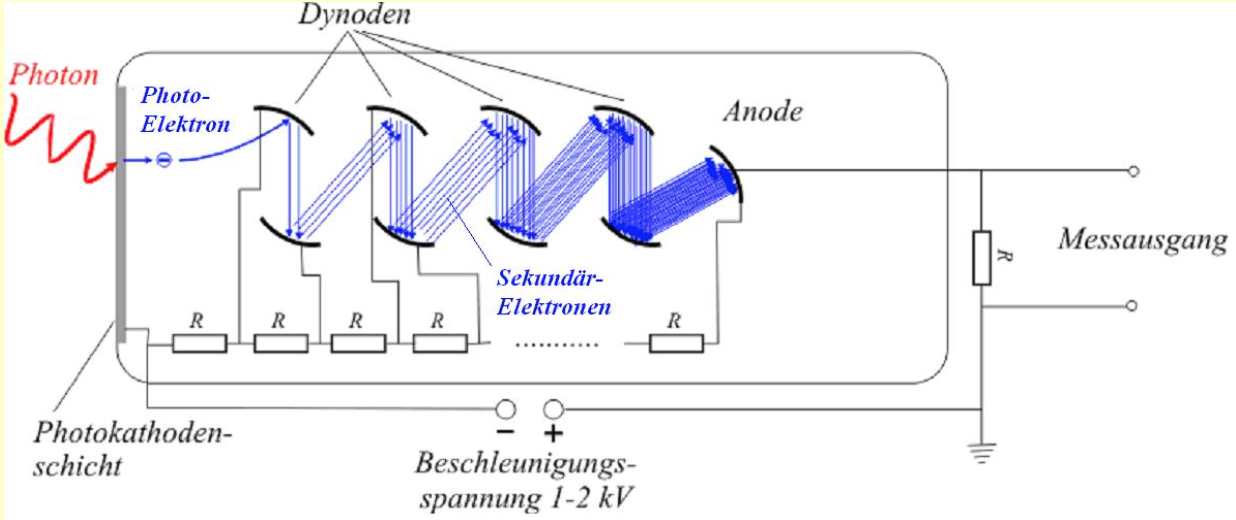
\includegraphics[scale=0.5]{resources/pmt.png}
  \caption{Schematischer Aufbau eines Photomultipliers \cite{pmt}.}
  \label{fig:03}
\end{figure}
\FloatBarrier
\noindent Zerfällt das Myon im Szintillatortank, wird von den dabei entstehenden
Elektronen oder Positronen ein gleichartiger Prozess ausgelöst. Der zeitliche
Abstand zwischen diesen Signalen kann dabei als Lebensdauer interpretiert werden,
sofern das Signal eindeutig vom Untergrund unterschieden werden kann. \\
\subsubsection{Bestimmung des Untergrunds}
\noindent Der Untergrund der Messung der Lebensdauer kosmischer Myonen besteht
aus den Myonen, welche im Szintillatortank detektiert werden, allerdings nicht
im Szintillatortank zerfallen. Mit der Annahme eines auf die Erdoberfläche
auftreffenden Myons pro $\si{\centi\meter^2}$ auf Meereshöhe pro Minute
\cite{grupen} und einem Szintillatortank mit einem Volumen $V = \SI{50}{\liter}$
und einem Verhältnis von Höhe  $h = 2 \cdot r$ \cite{anleitung} ergibt sich eine
Querschnittsfläche parallel zur Erdoberfläche von \\
\begin{align}
  A = 4 \cdot r \qquad \text{mit} \qquad r = \sqrt[3]{\frac{V}{2 \cdot \pi}}
  \label{eqn:03}
\end{align}
\begin{align*}
  \implies A \approx \SI{0.16}{\meter^2},
\end{align*}
\noindent was auf eine Ereignisrate im Szintillator von etwa $n = \num{1600}$
Ereignissen pro Minute schließen lässt. Diese Untergrundrate lässt auf ein
Zeitintervall von etwa $t_0 = \SI{37.5}{\milli\second}$ zwischen den Ereignissen
schließen, in welchem keine Signale registriert werden. \\
\newline
\noindent Ist die Zeitspanne zwischen den Signalen deutlich kürzer, ist ein
Myonenzerfall wahrscheinlich. Ein Photon im Szintillator wird dabei vom Myon
erzeugt, ein weiteres vom Elektron (bzw. Positron), welches beim Myonenzerfall
entsteht. Zu registrieren gilt es daher diese Zeitspanne. \\
